\documentclass[crop,tikz]{standalone}
\usetikzlibrary{backgrounds}
\colorlet{blue}{cyan}
\tikzset{
  inverted/.style = {
    color=white,
    background rectangle/.style={fill},
    show background rectangle
  }
}

\usepackage{pgfplots}
\usetikzlibrary{angles}

\tikzset{>=latex}

\pgfplotsset{
  every non boxed x axis/.append style={
    axis line style={-latex}
  },
  every non boxed y axis/.append style={
    axis line style={-latex}
  },
  inverted/.style = {
    every axis legend/.append style={
      draw=white,
      fill=white,
      text=white
    }
  }
}

\begin{document}
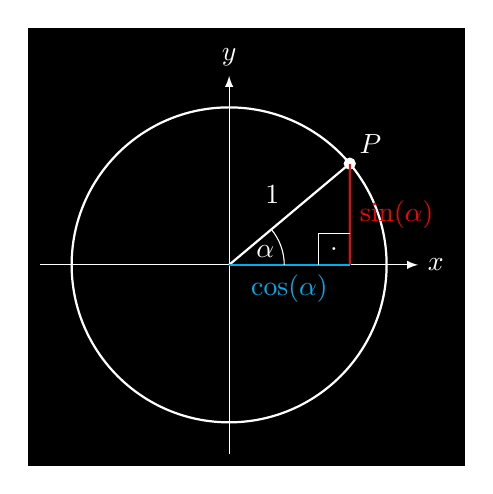
\begin{tikzpicture}[inverted,scale=2]
  \draw[->] (-1.2,0) -- (1.2,0) node[right] {$x$};
  \draw[->] (0,-1.2) -- (0,1.2) node[above] {$y$};
  \draw[thick] (0,0) circle (1);
  \coordinate (o) at (0,0);
  \coordinate (p) at (40:1);
  \coordinate (x) at (p |- o);
  \draw[fill] (p) circle (1pt);
  \draw[thick] (o) -- node[above left] {$1$} (p);
  \draw[thick,red] (p) -- node[right] {$\sin(\alpha)$} (x);
  \draw[thick,blue] (x) -- node[below] {$\cos(\alpha)$} (o);
  \node[above right] at (p) {$P$};
  \pic[draw, angle eccentricity=0.7, angle radius=0.7cm, pic text={$\alpha$}] {angle = x--o--p};
  \pic[draw, angle eccentricity=0.5, angle radius=0.4cm, pic text=.] {right angle = p--x--o};
\end{tikzpicture}
\end{document}
